\problemname{Train Switching}

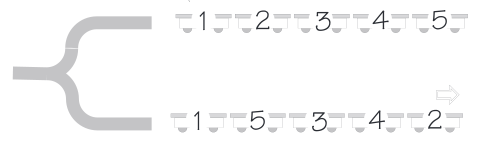
\includegraphics{tag.png}

On the top track (called the input track) there is a train with $n$ cars, numbered from 1 to $n$ starting from the front car.
On the lower track (called the output track) you see the same cars in the desired order as the train leaves the switching area.

The order of the cars can be changed by pushing them onto the siding (which is long enough to hold all cars at once). Only two movements are allowed:

\begin{itemize}
\item The first car on the input track to the last position on the siding
\item The last car on the siding to the last position on the output track
\end{itemize}
Write a program that receives the desired order on the output track and determines whether this order is possible to achieve. The order of the $n$ cars on the input track is always in ascending numerical order from first to last car.

\section*{Input}
The first line of input contains the integer $n$ ($1 \leq n \leq 100$),
the number of train cars.

The next line contains the integers $g_1, g_2, \dots, g_n$ ($1 \leq g_i \leq n$),
the desired order of the cars.
It is guaranteed that all $g_i$ are unique.

\section*{Output}
If it is possible to reach the desired arrangement, print \texttt{JA}. Otherwise, print \texttt{NEJ}.
